\documentclass{pginz}
%%%%%%%%%Miejsce na dodatkowe pakiety%%%%%%%%%%%%%
\usepackage{subcaption}
\PassOptionsToPackage{polish}{babel}
\usepackage{babel}
\usepackage[utf8]{inputenc}  % For UTF-8 support
\usepackage{tikz}
\usepackage{circuitikz}
\usepackage{algorithm}
\usepackage{algpseudocode}
\usepackage{pgfplots}
\pgfplotsset{compat=1.18}
\usepackage[T1]{fontenc}
\usepackage{lmodern}
\usepackage{mathpazo}
\usepackage{textcomp}
\DeclareTextSymbol{\textOslash}{T1}{216}
\newcommand{\Oslash}{\textOslash}
\usepackage{url}
\urlstyle{same}


\begin{document}

\includepdf{assets/StronaTytulowa.pdf}
%\includepdf[page={1}]{Oswiadczenie.pdf}

\setcounter{page}{2}

%\chapter*{Streszczenie}

\noindent\textbf{Dziedzina nauki i techniki zgodna z OECD} Nauki inżynieryjne i techniczne, Elektrotechnika, elektronika i inżynieria informatyczna, Robotyka i Automatyka


%\chapter*{Abstract}

\noindent\textbf{Reinforcement learning for the Super Mario Bros. game}
The aim of this engineering thesis was to develop and evaluate a reinforcement learning-based model capable of completing levels in the \textit{Super Mario Bros} game. The implementation utilized the Double Q-Learning algorithm, a convolutional neural network, and the Weights and Biases tool for experiment monitoring. The thesis analyzed the impact of training parameters, such as the discount factor, epsilon decay strategy, and reward function, on model performance. The results confirm that appropriate parameter tuning and a balanced reward function significantly enhance the algorithm's efficiency.


\tableofcontents
\addcontentsline{toc}{chapter}{Spis treści}

%\chapter*{Lista symboli}

\begin{itemize}[noitemsep,topsep=0pt,parsep=0pt,partopsep=0pt,labelwidth=1cm,align=left,itemindent=0pt]
\item[$\mathbf{u}$] - wejście systemu
\item[$\mathbf{Q}_c$] - macierz kowariancji
\item[$F$] - napięcie $\left[ \frac{kg \cdot m}{s^2} \right]$ %\si[per-mode=fraction]{\kilo\gram\meter\per\second\squared}
\item[$R$] - rezystancja [\si{\ohm}]
\end{itemize}
%\chapter*{Lista skrótów}

\begin{itemize}[noitemsep,topsep=0pt,parsep=0pt,partopsep=0pt,labelwidth=1cm,align=left,itemindent=0pt]
\item[SD] - Systemy Diagnostyki
\item[EKF] - Rozszerzony filtr Kalmana (ang. \textit{Extended Kalman Filter})
\end{itemize}

\chapter{Wstęp}

\section{Cel pracy}
Celem projektu inżynierskiego jest opracowanie programu opartego na uczeniu maszynowym, zdolnego do samodzielnego rozwiązywania problemów występujących w grze \textit{Super Mario Bros} na platformie Nintendo Entertainment System (NES).
Projekt obejmuje badanie zastosowania algorytmów uczenia ze wzmocnieniem oraz analizę efektywności różnych podejść w symulowanym środowisku gry.

\section{Opis gry \textit{Super Mario Bros}}

\textit{Super Mario Bros} to klasyczna gra platformowa wydana przez Nintendo w 1985 roku na konsolę NES.
Celem gry jest przejście bohaterem, Mario, z lewej strony ekranu na prawą, aż do końca poziomu, gdzie zwykle znajduje się flaga oznaczająca jego ukończenie.
Gracz musi pokonać serię poziomów.

Podczas gry Mario napotyka różnorodne przeszkody, wrogów oraz pułapki.
Do głównych zagrożeń należą przeciwnicy, tacy jak Goomba i Koopa Troopa, przepaście oraz spadające platformy.
Aby unikać zagrożeń lub je eliminować, Mario może skakać na wrogów lub korzystać z przedmiotów zwiększających jego zdolności, takich jak grzyby, które powiększają postać, czy kwiaty ognia umożliwiające atakowanie przeciwników z dystansu.

Kluczową mechaniką gry jest precyzyjne poruszanie się i planowanie kolejnych ruchów, ponieważ niewłaściwe decyzje często prowadzą do przegranej.

\begin{figure}[h!]
    \centering
    \includegraphics[width=0.8\textwidth]{img/screenshot_mario.png}
    \caption{Przykładowy ekran z gry \textit{Super Mario Bros.}}
    \label{fig:screenshot_mario}
\end{figure}

\subsection{Kontroler NES}

Do gry wykorzystywany jest prosty kontroler NES. Posiada on cztery przyciski kierunkowe (góra, dół, lewo, prawo) oraz dwa przyciski akcji oznaczone jako \textit{A} i \textit{B}. Przyciski te pozwalają na wykonywanie takich czynności jak skakanie, bieganie i atakowanie przeciwników.


\begin{figure}[h!]
    \centering
    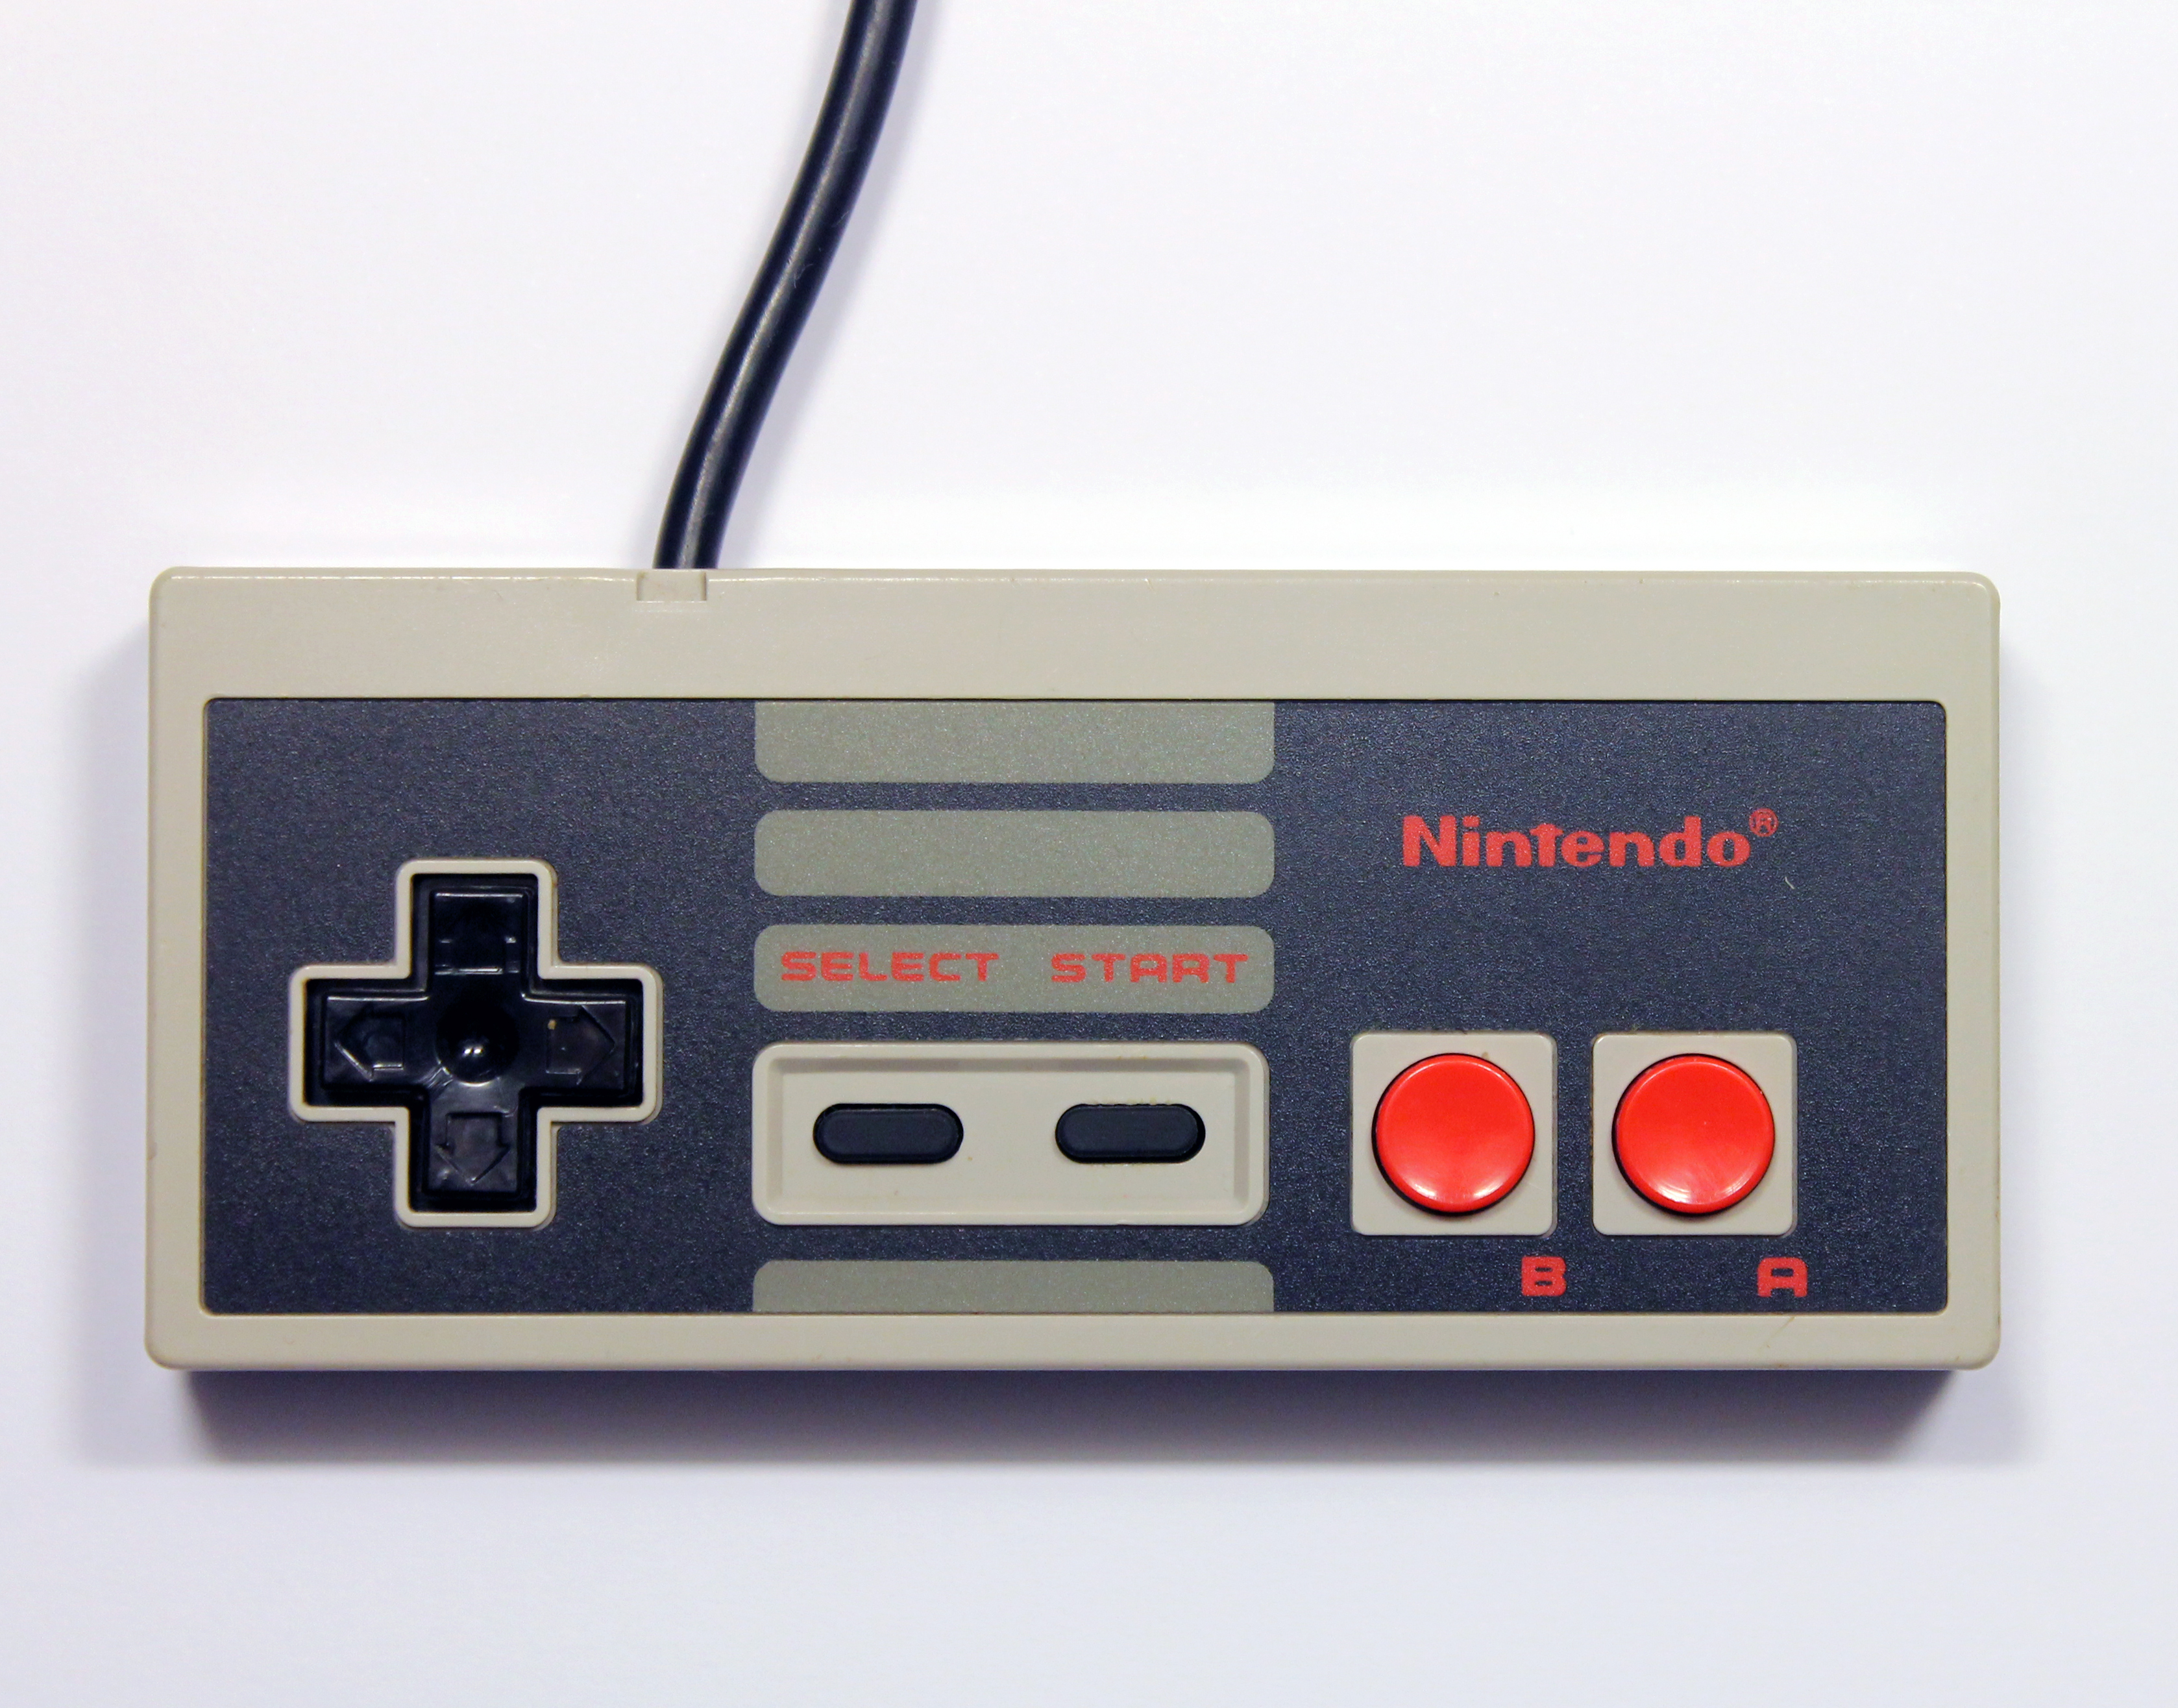
\includegraphics[width=0.5\textwidth]{img/nes_controller.JPG}
    \caption{Kontroler NES używany w grze Super Mario Bros.\\Denis Apel / \url{flyingpixel.de} / Wikipedia}
    \label{fig:nes_controller}
\end{figure}

\section{Zakres pracy}
Celem niniejszej pracy jest stworzenie programu, który nauczy model sztucznej inteligencji skutecznego przechodzenia wybranego poziomu gry Super Mario Bros. Projekt obejmuje:
\begin{itemize}
    \item opracowanie środowiska umożliwiającego interakcję z emulatorem NES,
    \item implementację algorytmu Double Q-Learning,
    \item przeprowadzenie eksperymentów oceniających efektywność modelu.
\end{itemize}
Zakres pracy ogranicza się do jednego wybranego poziomu gry, z pominięciem aspektów dźwięku oraz rozgrywki wielopoziomowej.

\chapter{Wstęp i cel pracy}



\chapter{Projekt systemu}

\section{Ogólna architektura systemu}

System został zaprojektowany w celu nauki agenta, który skutecznie przechodzi poziomy w grze Super Mario Bros, wykorzystując algorytm Double Q-Learning. Architektura systemu składa się z czterech głównych komponentów: emulatora NES, agenta, algorytmu trenującego (DQN) oraz mechanizmu agregacji danych.

\subsection{Emulator NES}

Środowisko gry zostało zaimplementowane przy użyciu emulatora NES opartego na bibliotece \texttt{cynes} \cite{CYNES}. Emulator dostarcza informacje o stanie gry poprzez odczyt pamięci RAM oraz renderowanie obrazu gry w czasie rzeczywistym.

\subsection{Agent}

Agent w systemie to model decyzyjny, który podejmuje akcje w środowisku gry na podstawie bieżącego stanu. Model ten jest trenowany za pomocą algorytmu Double Q-Learning. Agent:

\begin{itemize}
	\item \textbf{Wejście:} Otrzymuje przetworzony obraz, generowany przez emulator \texttt{cynes}.
	\item \textbf{Wyjście:} Generuje sześć wartości odpowiadających naciśniętym klawiszom:
	      \begin{itemize}
		      \item cztery kierunki ruchu (lewo, prawo, góra, dół),
		      \item dwa przyciski akcji (A i B).
	      \end{itemize}
	\item \textbf{Cel:} Nauka optymalnej strategii, która maksymalizuje sumę nagród za pomocą algorytmu Double Q-Learning.
\end{itemize}
\subsection{Agregacja danych}

Mechanizm agregacji danych zajmuje się odczytem istotnych informacji ze stanu pamięci emulatora, takich jak pozycja Mario, prędkość, aktualny poziom, liczba punktów, a także stan przeciwników. Dane te są później używane do trenowania agenta. Tabela~\ref{tab:nes_memory} przedstawia najważniejsze zmienne i ich adresy w pamięci RAM.

\begin{table}[ht]
	\centering
	\caption{Zmienne odczytywane z pamięci emulatora NES}
	\label{tab:nes_memory}
	\begin{tabular}{|c|c|p{5cm}|}
		\hline
		\textbf{Adres w RAM}      & \textbf{Nazwa zmiennej}          & \textbf{Opis}                                         \\ \hline
		\texttt{0x75A}            & \texttt{lives}                   & Liczba żyć Mario.                                     \\ \hline
		\texttt{0x006D}           & \texttt{x\_horizontal}           & Pozioma pozycja Mario (wysoki bajt).                  \\ \hline
		\texttt{0x0086}           & \texttt{x\_on\_screen}           & Pozioma pozycja Mario na ekranie (niski bajt).        \\ \hline
		\texttt{0x0057}           & \texttt{horizontal\_speed}       & Prędkość pozioma Mario (w postaci liczby ze znakiem). \\ \hline
		\texttt{0x00CE}           & \texttt{y\_position\_on\_screen} & Pionowa pozycja Mario na ekranie.                     \\ \hline
		\texttt{0x0760}           & \texttt{level}                   & Aktualny numer poziomu gry.                           \\ \hline
		\texttt{0x07DD do 0x07E2} & \texttt{score\_bcd}              & Wynik punktowy w formacie BCD (Binary-Coded Decimal). \\ \hline
	\end{tabular}
\end{table}
\subsection{Przepływ danych w systemie}

\begin{figure}
	\begin{center}
		\begin{tikzpicture}[node distance=1.0cm]
			\node[draw, rectangle, minimum width=4cm, minimum height=0.7cm] (input) {Wejście: [60x64]};
			\node[draw, rectangle, minimum width=4cm, minimum height=0.7cm, below of=input] (conv1) {Warstwa konwolucyjna: 1 $\rightarrow$ 32};
			\node[draw, rectangle, minimum width=4cm, minimum height=0.7cm, below of=conv1] (bn1) {Warstwa normalizująca: 64 kanały};
			\node[draw, rectangle, minimum width=4cm, minimum height=0.7cm, below of=bn1] (conv2) {Warstwa konwolucyjna: 32 $\rightarrow$ 64};
			\node[draw, rectangle, minimum width=4cm, minimum height=0.7cm, below of=conv2] (bn2) {Warstwa normalizująca: 64 kanały};
			\node[draw, rectangle, minimum width=4cm, minimum height=0.7cm, below of=bn2] (flatten) {Spłaszczenie: 1x30720};
			\node[draw, rectangle, minimum width=4cm, minimum height=0.7cm, below of=flatten] (fc1) {Warstwa gęsta: 30720 $\rightarrow$ 128};
			\node[draw, rectangle, minimum width=4cm, minimum height=0.7cm, below of=fc1] (fc2) {Warstwa gęsta: 128 $\rightarrow$ 6};
			\node[draw, rectangle, minimum width=4cm, minimum height=0.7cm, below of=fc2] (output) {Wyjście: 6 wartości};

			% Connections
			\draw[->] (input) -- (conv1);
			\draw[->] (conv1) -- (bn1);
			\draw[->] (bn1) -- (conv2);
			\draw[->] (conv2) -- (bn2);
			\draw[->] (bn2) -- (flatten);
			\draw[->] (flatten) -- (fc1);
			\draw[->] (fc1) -- (fc2);
			\draw[->] (fc2) -- (output);

		\end{tikzpicture}
	\end{center}
\end{figure}

\begin{itemize}
	\item Agent odczytuje aktualny stan gry z pamięci emulatora, w tym pozycję Mario, liczbę żyć, prędkość i wynik.
	\item Na podstawie obrazu gry i odczytanych danych agent wybiera akcję za pomocą strategii \(\epsilon\)-greedy.
	\item Akcja jest przekazywana do emulatora w formie naciśniętych klawiszy.
	\item Emulator aktualizuje stan gry i zwraca wynikowe dane, które są zapisywane przez mechanizm agregacji.
\end{itemize}
\begin{figure}[ht]
	\begin{center}
		\resizebox{\textwidth}{!}{
			\begin{tikzpicture}[
					node distance=2.5cm, % Odstęp między węzłami
					align=center, % Wyśrodkowanie tekstu w węzłach
					>=latex, % Strzałki w stylu LaTeX
					%every node/.style={draw, text width=3cm} % Styl węzłów
				]

				\node[rectangle, minimum width=5cm, draw=black] (full_frame) {\includegraphics[width=4cm]{img/full_frame.png}\\Obraz generowany przez emulator NES};

				\node[right of=full_frame, xshift=6cm, draw=black] (compressed_frame) {\includegraphics[width=2.5cm]{img/compressed_frame.png} \\Skompresowany obraz};
				\node (model) [right of=compressed_frame, draw = black, minimum height=2cm, xshift=2cm] {Model};

				\node (controller) [right of=model, draw=black, minimum height = 2cm, xshift=1cm, minimum width = 2cm] {Przyciski\\kontrolera\\NES};

				\draw[<-] (compressed_frame.west) -- (full_frame.east) node[midway] {Zmniejszenie\\ rozmiaru i \\ konwersja na skalę \\szarości};
				\draw[<-] (model.west) -- (compressed_frame.east) node[midway]{Konwersja\\na tensor};
				\draw[<-] (controller.west) -- (model.east) node[midway] {Predykcja\\wciśnięć};

			\end{tikzpicture}
		}
	\end{center}
	\caption{Ogólny schemat działania programu}
	\label{fig:sys_diagram}
\end{figure}

\chapter{Implementacja}

Implementacja projektu została zrealizowana przy użyciu kilku kluczowych technologii i narzędzi wspierających proces uczenia modelu oraz monitorowanie eksperymentów. Poniżej przedstawiono najważniejsze szczegóły implementacyjne oraz architekturę systemu.

\section{Technologie}

\begin{itemize}
	\item \textbf{PyTorch:} Biblioteka do budowy i trenowania modelu DQN (Deep Q-Network) oraz implementacji warstw konwolucyjnych, w pełni połączonych i mechanizmów propagacji gradientów.
	\item \textbf{Weights and Biases (WandB):} Narzędzie do monitorowania eksperymentów, umożliwiające śledzenie hiperparametrów, wyników oraz wizualizację metryk uczenia.
	\item \textbf{Własny algorytm DQN:} Algorytm Double Q-Learning został zaimplementowany ręcznie w celu lepszego dostosowania do specyficznych wymagań projektu.
\end{itemize}
\section{Architektura systemu}

Cały system został zaprojektowany do pracy na zdalnej maszynie wyposażonej w GPU NVIDIA, gdzie jednocześnie działa wiele procesów związanych z różnymi modelami. System korzysta z dodatkowych narzędzi, takich jak \texttt{WandB} do monitorowania i archiwizacji oraz \texttt{SQLite} do przechowywania parametrów modelu i stanu optymalizatora. Architektura systemu jest przedstawiona na rysunku~\ref{fig:system_architecture}.

\begin{figure}[h!]
	\resizebox{\textwidth}{!}{
		\centering
		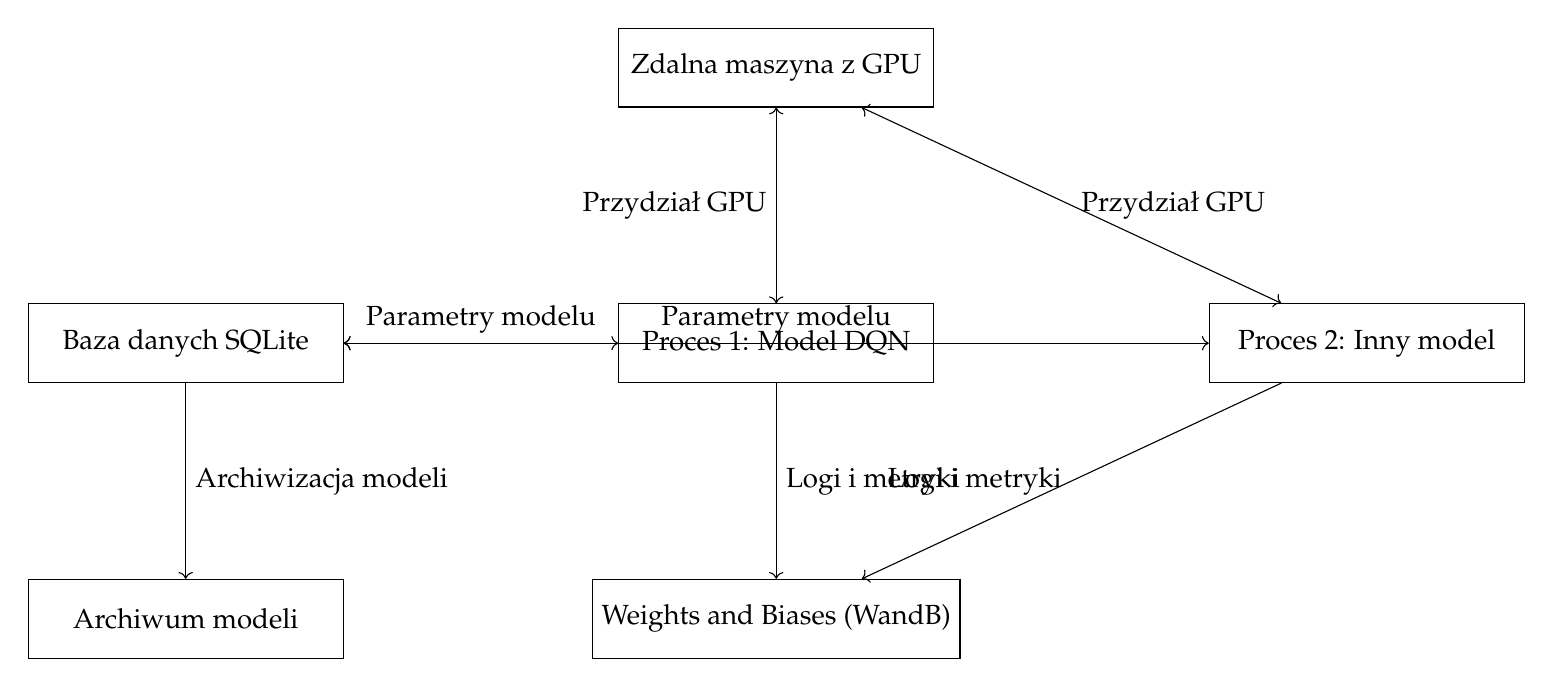
\begin{tikzpicture}[node distance=2.5cm]
			% Nodes
			\node[draw, rectangle, minimum width=4cm, minimum height=1cm] (gpu) {Zdalna maszyna z GPU};
			\node[draw, rectangle, minimum width=4cm, minimum height=1cm, below of=gpu, yshift=-1cm] (process1) {Proces 1: Model DQN};
			\node[draw, rectangle, minimum width=4cm, minimum height=1cm, right of=process1, xshift=5cm] (process2) {Proces 2: Inny model};
			\node[draw, rectangle, minimum width=4cm, minimum height=1cm, left of=process1, xshift=-5cm] (sqlite) {Baza danych SQLite};
			\node[draw, rectangle, minimum width=4cm, minimum height=1cm, below of=process1, yshift=-1cm] (wandb) {Weights and Biases (WandB)};
			\node[draw, rectangle, minimum width=4cm, minimum height=1cm, below of=sqlite, yshift=-1cm] (archive) {Archiwum modeli};

			% Arrows
			\draw[<->] (gpu) -- (process1) node[midway, left] {Przydział GPU};
			\draw[<->] (gpu) -- (process2) node[midway, right] {Przydział GPU};
			\draw[<->] (process1) -- (sqlite) node[midway, above] {Parametry modelu};
			\draw[<->] (process2) -- (sqlite) node[midway, above] {Parametry modelu};
			\draw[->] (process1) -- (wandb) node[midway, right] {Logi i metryki};
			\draw[->] (process2) -- (wandb) node[midway, left] {Logi i metryki};
			\draw[->] (sqlite) -- (archive) node[midway, right] {Archiwizacja modeli};
		\end{tikzpicture}
	}
	\caption{Architektura systemu implementacji}
	\label{fig:system_architecture}
\end{figure}

\section{Szczegóły implementacyjne}

\begin{itemize}
	\item \textbf{Zdalna maszyna z GPU:} System działa na serwerze wyposażonym w GPU NVIDIA, umożliwiając równoczesne trenowanie kilku modeli. GPU przydzielane są do poszczególnych procesów w zależności od obciążenia.
	\item \textbf{Weights and Biases (WandB):} WandB jest używane do monitorowania eksperymentów. Zapisuje logi, metryki (np. stratę i nagrody) oraz regularnie archiwizuje stany modelu i optymalizatora.
	\item \textbf{SQLite:} Lekka baza danych SQLite przechowuje parametry modelu, stany optymalizatora oraz inne dane konfiguracyjne, co umożliwia łatwe wznowienie treningu lub analizę po zakończeniu procesu.
	\item \textbf{Archiwum modeli:} Modele i stany optymalizatora są regularnie zapisywane w formacie binarnym w lokalnym archiwum, co pozwala na późniejsze wykorzystanie i ewaluację.
	\item \textbf{Procesy równoległe:} Na maszynie uruchamiane są równocześnie różne procesy, z których każdy zajmuje się trenowaniem innego modelu. WandB synchronizuje dane z każdego procesu w czasie rzeczywistym.
\end{itemize}

\section{Monitorowanie i archiwizacja}

Dzięki integracji z WandB i SQLite proces treningu jest w pełni monitorowany. WandB umożliwia wizualizację wyników w czasie rzeczywistym, a SQLite zapewnia
\section{Uruchomienie systemu}

System działa na zdalnej maszynie, co wymaga:
\begin{itemize}
	\item Konfiguracji środowiska wirtualnego z bibliotekami \texttt{PyTorch}, \texttt{WandB} oraz dodatkowymi zależnościami.
	\item Połączenia z serwerem WandB w celu monitorowania eksperymentów.
	\item Uruchomienia emulatora NES i algorytmu DQN na zdalnej maszynie wyposażonej w GPU.
\end{itemize}

Proces treningu obejmuje iteracyjne aktualizowanie modelu DQN, przesyłanie wyników do WandB oraz przechowywanie danych w Replay Buffer w celu stabilizacji procesu uczenia.

\chapter[Przegląd literatury]{PrzeglĄd literatury}
\label{chap:przeglad}
Uczenie ze wzmocnieniem (ang. Reinforcement Learning, RL) jest jednym z najważniejszych podejść do sztucznej inteligencji, szczególnie w kontekście sterowania agentami w złożonych środowiskach, takich jak gry wideo. W literaturze naukowej można znaleźć liczne prace badające różne aspekty i ulepszenia algorytmów RL, które w znaczący sposób przyczyniły się do rozwoju tej dziedziny. W szczególności, prace poświęcone grze Super Mario Bros oraz innym platformom do gier, takim jak Atari czy Nintendo Entertainment System (NES), pozwalają lepiej zrozumieć wyzwania stojące przed algorytmami RL.

W pracy LeBlanca i Lee \cite{NES} autorzy badali zastosowanie uczenia ze wzmocnieniem wśrodowisku konsoli do gier NES. Autorzy wykorzystali agentów RL, którzy byli trenowani bez dostarczania wiedzy eksperckiej, co pozwoliło na zbadanie, jak dobrze nowoczesne algorytmy są w stanie sobie radzić w środowiskach o dużym stopniu złożoności. W pracy omówiono zmiany w hiperparametrach i funkcjach nagród, które są niezbędne do skutecznego rozwiązania problemów w grach NES, wykorzystując dane pikselowe jako jedyne wejście do sieci neuronowych agentów.

Hessel i współpracownicy \cite{RAI} przeanalizowali szereg niezależnych ulepszeń algorytmu DQN (Deep Q-Network), które wprowadzono w ostatnich latach w społeczności zajmującej się uczeniem ze wzmocnieniem. W pracy połączono sześć kluczowych rozszerzeń DQN, które wcześniej były badane oddzielnie, aby ocenić ich komplementarność. Wyniki eksperymentów przeprowadzonych na konsoli Atari 2600 wykazały, że połączenie tych ulepszeń skutkuje znacznym zwiększeniem efektywności algorytmu zarówno pod względem wydajności danych, jak i ostatecznej jakości wyników.

Salimans i inni \cite{EV} przedstawili alternatywne podejście do metod opartych na procesach decyzyjnych Markowa (MDP), takich jak Q-learning i Policy Gradients, poprzez zastosowanie strategii ewolucyjnych (ES). ES, jako technika optymalizacji „czarnej skrzynki”, charakteryzuje się dużą skalowalnością w zależności od liczby dostępnych jednostek obliczeniowych (CPU). W pracy wykazano, że zastosowanie tej metody umożliwia równoległe trenowanie agentów na dużą skalę, co pozwala na szybkie rozwiązywanie złożonych problemów, takich jak poruszanie się humanoida w symulatorze 3D w 10 minut oraz osiągnięcie konkurencyjnych wyników w większości gier Atari po godzinie treningu. ES wykazuje również tolerancję na długie horyzonty czasowe oraz niewrażliwość na częstotliwość akcji i opóźnione nagrody, co jest istotne w grach o dużej złożoności, takich jak Super Mario Bros.

Van Hasselt i współautorzy \cite{DQ} skoncentrowali się na problemie przeszacowania wartości akcji w popularnym algorytmie Q-learning, który może prowadzić do gorszej wydajności w pewnych warunkach. Autorzy przedstawili algorytm Double Q-learning, który redukuje ten problem, oddzielając wybór akcji od jej oceny. Zastosowanie tej techniki w algorytmie DQN pozwoliło na znaczne zmniejszenie przeszacowania wartości w grach Atari, co z kolei prowadziło do lepszych wyników w porównaniu do standardowego DQN.

Na koniec, książka Gérona \cite{HML} dostarcza kompleksowego omówienia technik uczenia maszynowego, w tym uczenia ze wzmocnieniem, z naciskiem na narzędzia takie jak Scikit-Learn i TensorFlow. Książka ta stanowi doskonałe źródło wiedzy dla inżynierów i badaczy, którzy chcą wdrożyć nowoczesne techniki uczenia maszynowego, w tym RL, do rzeczywistych systemów, takich jak gry wideo.


% tu będą kolejne rozdziały

%\listoffigures
%\addcontentsline{toc}{chapter}{Spis rysunków}
%\listoftables
%\addcontentsline{toc}{chapter}{Spis tabel}
\begin{thebibliography}{99}
	\bibitem{DQ}
	Hasselt H., Guez A., Silver D.:
	\emph{Deep Reinforcement Learning with Double Q-learning},
	\url{https://doi.org/10.48550/arXiv.1509.06461},
	Google Deep Mind, 2015.

	\bibitem{NES}
	LeBlanc D. G., Lee G.:
	\emph{General Deep Reinforcement Learning in NES Games},
	\url{https://doi.org/10.21428/594757db.8472938b},
	Canadian Artificial Intelligence Association (CAIAC), 2021.

	\bibitem{EV}
	Salimans T., Ho J., Chen X., Sidor S., Sutskever I.:
	\emph{Evolution Strategies as a Scalable Alternative to Reinforcement Learning},
	\url{https://doi.org/10.48550/arXiv.1703.03864}, OpenAI, 2017.

	\bibitem{RAI}
	Hessel M., Modayil J., van Hasselt H., Schaul T., Ostrovski G., Dabney W., Horgan D., Piot B., Gheshlaghi Azar M., Silver D.:
	\emph{Rainbow: Combining Improvements in Deep Reinforcement Learning},
	\url{https://doi.org/10.48550/arXiv.1710.02298},
	Google Deep Mind, 2017.

	\bibitem{HML}
	Géron A.:
	\emph{Hands-On Machine Learning with Scikit-Learn and TensorFlow: Concepts, Tools, and Techniques to Build Intelligent Systems},
	O'Reilly Media, 2017.

	\bibitem{VIME} Houthooft, R., Chen, X., Duan, Y., Schulman, J., De Turck, F., Abbeel, P.: \emph{VIME: Variational Information Maximizing Exploration},  \url{https://doi.org/10.48550/arXiv.1605.09674}, OpenAI, 2017.

	\bibitem{GRAD} Silver, D., Lever, G., Heess, N., Degris, T., Wierstra, D., Riedmiller, M.: \emph{Deterministic Policy Gradient Algorithms}, 31st International Conference on Machine Learning, ICML 2014.

	\bibitem{BELLEMARE2013}
	Bellemare M., Naddaf Y., Veness J., Bowling M.:
	\emph{The Arcade Learning Environment: An Evaluation Platform for General Agents},
	\url{https://doi.org/10.5555/3042817.3042830},
	University of Alberta, 2013.

	\bibitem{KARPATHY2015}
	Karpathy A.:
	\emph{Deep Reinforcement Learning: Pong from Pixels},
	\url{http://karpathy.github.io/2016/05/31/rl/},
	Stanford University, 2015.

	\bibitem{BROCKMAN2016}
	Brockman G., Cheung V., Pettersson L., Schneider J., Schulman J., Tang J., Zaremba W.:
	\emph{OpenAI Gym},
	\url{https://doi.org/10.48550/arXiv.1606.01540},
	OpenAI, 2016.

	\bibitem{KEMPKA2016}
	Kempka M., Wydmuch M., Runc G., Toczek J., Jaśkowski W.:
	\emph{ViZDoom: A Doom-based AI Research Platform for Visual Reinforcement Learning},
	\url{https://doi.org/10.48550/arXiv.1605.02097},
	Politechnika Poznańska, 2016.

	\bibitem{TODOROV2012}
	Todorov E., Erez T., Tassa Y.:
	\emph{MuJoCo: A Physics Engine for Model-Based Control},
	\url{https://doi.org/10.1109/IROS.2012.6386109},
	University of Washington, 2012.

	\bibitem{SCHULMAN2017}
	Schulman J., Wolski F., Dhariwal P., Radford A., Klimov O.:
	\emph{Proximal Policy Optimization Algorithms (Roboschool)},
	\url{https://doi.org/10.48550/arXiv.1707.06347},
	OpenAI, 2017.

	\bibitem{COUMANS2016}
	Coumans E.:
	\emph{PyBullet, a Python module for physics simulation in robotics},
	\url{http://pybullet.org},
	2016.

	\bibitem{DOSOVITSKIY2017}
	Dosovitskiy A., Ros G., Codevilla F., Lopez A., Koltun V.:
	\emph{CARLA: An Open Urban Driving Simulator},
	\url{https://doi.org/10.48550/arXiv.1711.03938},
	Intel Labs, 2017.

	\bibitem{SUTTON2018}
	Sutton R., Barto A.:
	\emph{Reinforcement Learning: An Introduction (2nd Edition)},
	\url{https://doi.org/10.1201/9781315361564},
	MIT Press, 2018.

	\bibitem{RUSSELL2003}
	Russell S., Norvig P.:
	\emph{Artificial Intelligence: A Modern Approach (2nd Edition)},
	\url{https://doi.org/10.5555/3000006},
	Stanford University, 2003.

	\bibitem{PUTERMAN1994}
	Puterman M. L.:
	\emph{Markov Decision Processes: Discrete Stochastic Dynamic Programming},
	\url{https://doi.org/10.1002/9781118625776},
	Wiley, 1994.

	\bibitem{CYNES}
	Combey T.:
	\emph{cynes - C/C++ NES emulator with Python bindings},
	\url{https://github.com/Youlixx/cynes}.
	\bibitem{he2015}
	He K., Zhang X., Ren S., Sun J.:
	\emph{Delving Deep into Rectifiers: Surpassing Human-Level Performance on ImageNet Classification},
	\url{https://doi.org/10.48550/arXiv.1502.01852},
	IEEE International Conference on Computer Vision (ICCV), 2015.
	\bibitem{krogh1992}
	Krogh A., Hertz J. A.:
	\emph{A Simple Weight Decay Can Improve Generalization},
	\url{https://doi.org/10.1016/0893-6080(92)90008-M},
	Neural Computation, 1992.
\end{thebibliography}



% spis rysunków
\chapter{Wykaz rysunków}

1.2. Kontroler NES używany w grze Super Mario Bros. Denis Apel / flyingpixel.de / Wikipedia, Źródło: \url{https://commons.wikimedia.org/wiki/File:NES_controller.JPG}.


%*****************
%wymagane dodatki:
% Opis dyplomu
% Zawartość płyty CD
% Instrukcja dla projektanta
% Instrukcja dla użytkownika
\begin{appendices}
	%\chapter[Instrukcja dla użytkownika]{Instrukcja dla u\.Zytkownika}
	%\include{AppB}
\end{appendices}
%*****************

\end{document}

